\documentclass{article}
\usepackage{algorithm}
\usepackage{algorithmic}
\usepackage{amsmath}
\usepackage{amssymb}
\usepackage{booktabs}
\usepackage{caption}
\usepackage{CJKutf8}
%\usepackage{ctex}  %使用宏包(为了能够显示汉字)
%\usepackage{CJK}
\usepackage{diagbox}	%斜线表头
\usepackage{float}
\usepackage{geometry}
\usepackage{graphicx}
\usepackage{ulem}
\usepackage{geometry}
\usepackage{graphicx}
\usepackage{hyperref}
\usepackage{listings}
\usepackage{subfigure}%并排子图 共享标题 有子标题
\usepackage{textcomp}
\usepackage{url}
\usepackage{verbatim}%多行注释
\usepackage{xcolor}
%\usepackage{fontspec}
%\setmonofont{Consolas}
\linespread{2.0}


%\tiny
%\scriptsize
%\footnotesize
%\small
%\normalsize
%\large
%\Large
%\LARGE
%\huge
%\Huge

\geometry{a4paper, left = 1.5cm, right = 1.5cm, top = 1cm, bottom = 2cm}
\lstset{
    backgroundcolor=\color{red!5!green!5!blue!5},%代码块背景色为浅灰色
    rulesepcolor= \color{gray}, %代码块边框颜色
    breaklines=true,  %代码过长则换行
    numbers=left, %行号在左侧显示
    numberstyle= \small,%行号字体
    keywordstyle= \color{red},%关键字颜色
    commentstyle=\color{gray}, %注释颜色
    frame=shadowbox,%用方框框住代码块
    escapeinside=``%逃逸字符,用于在插入代码中输入中文
    }

%%%%%%%%%%%%%%%%%%%%%%%%%%%%%%%%%%%%%%%%%%%%%%%%%%%%%%%%%%%%%%%%%%%%%%%%%%%
\begin{document}
	\title{Report on HttpComponents}  %———总标题
	\begin{center}
		\huge Report on Httpcomponents\\
		\hspace*{\fill} \\ %空行
		\begin{CJK}{UTF8}{gbsn}
			\normalsize 张宇轩, 2017K8009908041\\
		\end{CJK}{}
	\end{center}
	\begin{figure}[H]
		\centering
		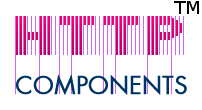
\includegraphics[height = 3.5cm, width = 5.5cm]{pics/1_httpcomponents.png}	
		%\caption{}
	\end{figure}

	\hspace*{\fill} \\ %空行
	
	\tableofcontents{} %—— 制作目录(目录是根据标题自动生成的)
	\clearpage
%%%%%%%%%%%%%%%%%%%%%%%%%%%%%%%%%% NEW PAGE %%%%%%%%%%%%%%%%%%%%%%%%%%%%%%%%%%%%%%%%%
	\section{Preface}
	\subparagraph{}
	\begin{CJK}{UTF8}{gbsn}
		由于先前的课程中并没有讲过关于网络与信息方面的知识,笔者之也并没有接触过。而这次的选题是HttpComponents,涉及到大量的网络方面的知识,所以在准备这篇报告的第一阶段笔者的主要精力是放在研究一些基本的网络方面的知识。要讲到HttpComponents,就先要讲一下关于http的各种知识。
	\end{CJK}{}
	\clearpage
	
	
	\section{The First Part}
	\paragraph{}
	\indent \indent 
	\begin{CJK}{UTF8}{gbsn}
		第一阶段解读的重点放在了连接http周边知识上。  
	\end{CJK}{}
	\subsection{Related Introduction}

	\subsubsection{http}
	\subparagraph{}
	%\indent \indent 
	\begin{CJK}{UTF8}{gbsn}
		从万维网(World Wide Web )服务器传输超文本到本地浏览器,基于请求与响应,无状态的,应用层的协议。
从本地角度去看http协议,就相当于浏览器访问一个url,然后就得到相应的web页面
从服务器角度去看http协议,就相当于客户端(浏览器)链接远程http服务器,服务器返回数据,浏览器接收、解析数据之后显示出来。 
	\end{CJK}{}
	\subsubsection{https}
	\subparagraph{}
	%\indent \indent 
	\begin{CJK}{UTF8}{gbsn}
		利用SSL(此处:基于应用层的访问控制)进行传输层加密的http传输协议,更加安全。\\ 
		https = http + SSL
	\end{CJK}{}
	\subsubsection{Proxy Server}
	\subparagraph{}
	\begin{CJK}{UTF8}{gbsn}
		代理服务器:代理个人网络从互联网服务商那里获取信息(通过在二者间建立非直接的连接),可以保证安全。
	\end{CJK}{}
	\subsubsection{Cookies}
	\subparagraph{}
	\begin{CJK}{UTF8}{gbsn}
		网站保存在用户端的含有用户信息以及行为的文本,用以弥补http协议的无状态性。举两个例子:
	\end{CJK}{}

	%\begin{comment}
	\begin{center}
	\fbox{
		\shortstack[l]{
	    	\begin{CJK}{UTF8}{gbsn}
				1.网站上的记住密码。网站将用户的身份和密码经过加密cookies存在用户硬盘中,下次登录的时候就不用手动输密码了。
			\end{CJK}{}\\
			\begin{CJK}{UTF8}{gbsn}
				2.上下文相关网址。如果上一个页面会对下一个页面产生影响,那次是就必须使用cookies。
			\end{CJK}{}\\
			\begin{CJK}{UTF8}{gbsn}
				比如一个购物网站,上一个页面选好商品,接下来的页面进行支付,支付页面就必须知道上一个页面中购买了什么东西,
			\end{CJK}{}\\
			\begin{CJK}{UTF8}{gbsn}
				此时就需要cookies。
			\end{CJK}{}
		}
	}
	\end{center}
	%\end{comment}

	\subsubsection{Request Format}
	\subparagraph{}
	\begin{CJK}{UTF8}{gbsn}
		客户端发送一个请求到服务器的请求消息格式如 Figure 1 所示(后面还会说到),请求头部的最后会有一个空行,表示请求头部结束,接下来为请求数据。
	\end{CJK}{}

	\begin{figure}[H]
		\centering
		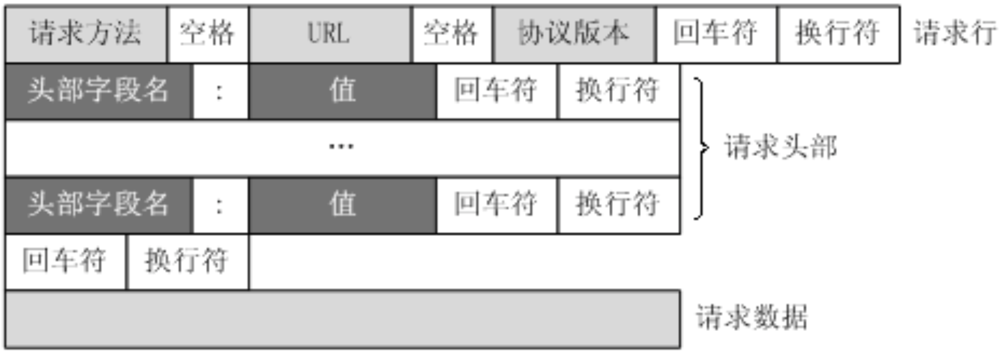
\includegraphics[height = 4.5cm, width = 12cm]{pics/2_request_format.png}	
		\caption{Request Format}
	\end{figure}
	\subsubsection{URL}
	\subparagraph{}
	\begin{CJK}{UTF8}{gbsn}
		URL(Uniform Resource Locator,统一资源定位符):一种资源位置的抽象唯一识别方法。\\
		URL组成:$<$协议$>$://$<$主机$>$:$<$端口$>$/$<$路径$>$ (端口和路径可以省略,端口默认80),如 Figure 2 所示: \\
		另外需要注意URI(Uniform Resource Identifier,统一资源标识符),用来表示web上每一种可用的资源,与URL不一样。 
	\end{CJK}{}
	\begin{figure}[H]
		\centering
		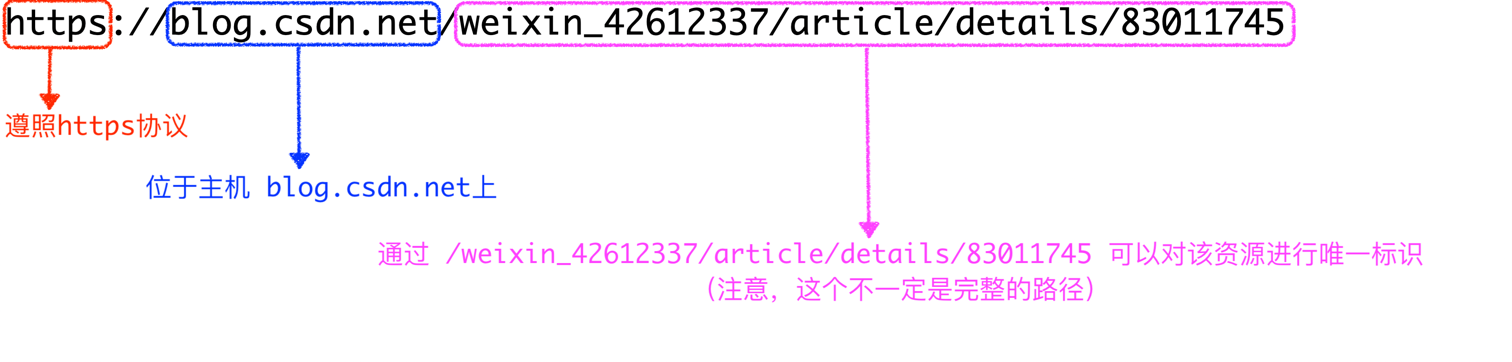
\includegraphics[height = 3.5cm, width = 16cm]{pics/3_url.png}	
		\caption{Request Format}
	\end{figure}

	\subsubsection{Http Request Methods}
	\subparagraph{}
	\begin{CJK}{UTF8}{gbsn}
		Http 协议共有9种请求方法,如 Figure 3 所示,其中最常用的两种方法是 GET 和 POST,其对比如 Figure 4 所示。\\
		GET - 从指定的资源请求数据。\\
		POST - 向指定的资源提交要被处理的数据。
	\end{CJK}{}
	\begin{figure}[H]
		\centering
		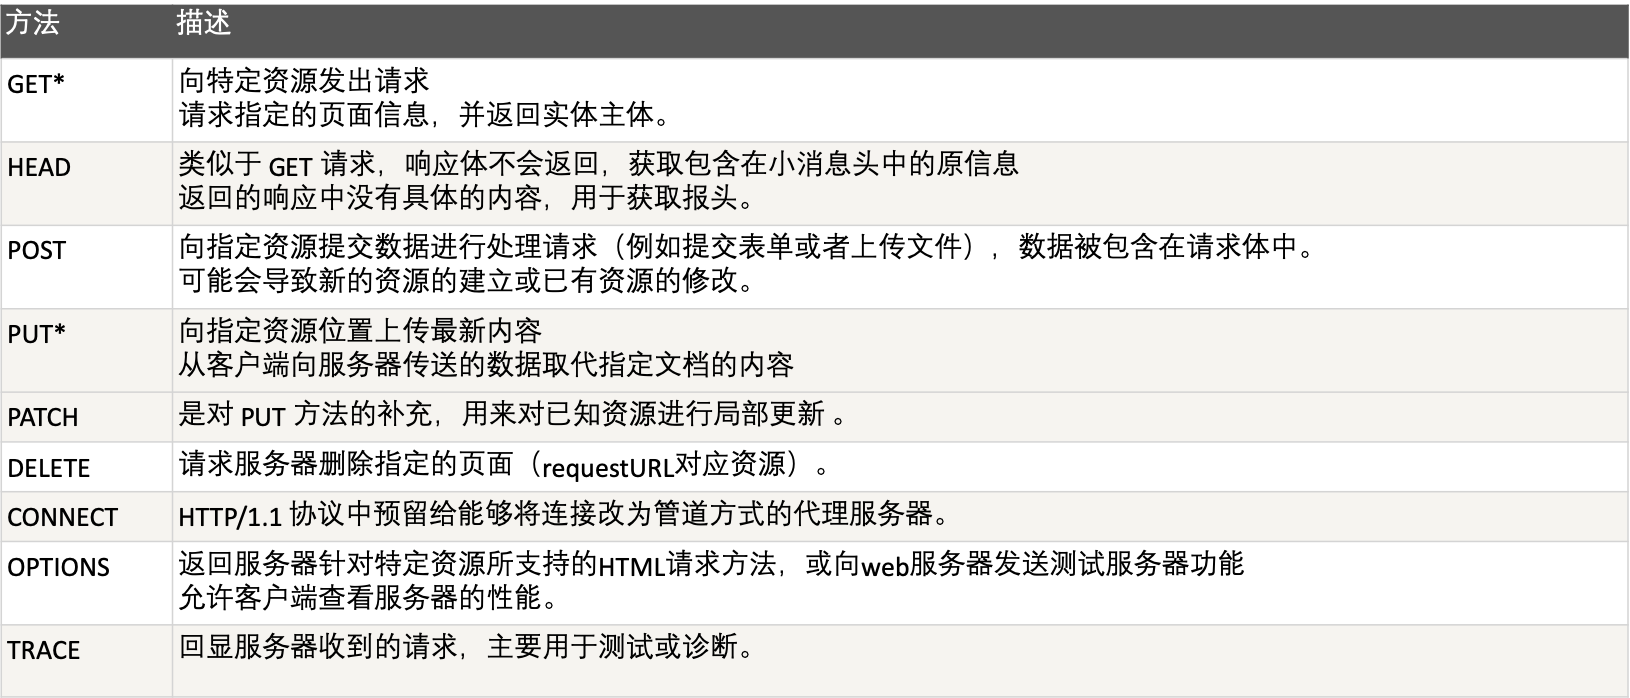
\includegraphics[height = 7.6cm, width = 16cm]{pics/4_9ways_of_http_request.png}	
		\caption{Request Format}
	\end{figure}
	\begin{figure}[H]
		\centering
		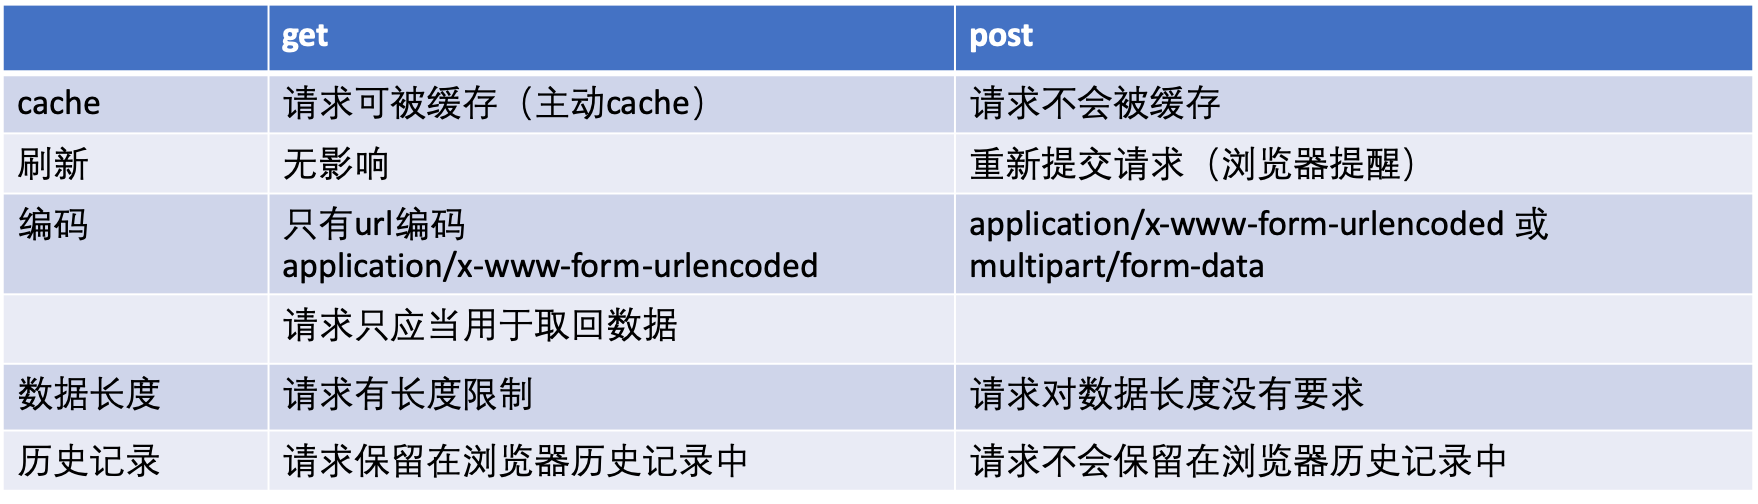
\includegraphics[height = 4.8cm, width = 15cm]{pics/5_get_post.png}	
		\caption{Get and Post}
	\end{figure}
	\begin{CJK}{UTF8}{gbsn}
		本文要介绍的HttpComponents就是用于提供对于http服务器的访问功能。
	\end{CJK}{}
	\subsection{About HttpComponents}
	%\subparagraph{}
	\begin{CJK}{UTF8}{gbsn}
		\subparagraph{}
		HttpComponents:用于提供对于http服务器的访问功能的超文本传输协议,其对HTTP底层协议进行了很好的封装。
		\subparagraph{}
		在构建HTTP客户端或者服务器端应用中很常见,比如WEB浏览器、爬虫、HTTP代理、WEB服务库、基于调整或扩展HTTP协议的分布式通信系统 etc.  
	\end{CJK}{}
	\clearpage
%%%%%%%%%%%%%%%%%%%%%%%%%%%%%%%%%% NEW PAGE %%%%%%%%%%%%%%%%%%%%%%%%%%%%%%%%%%%%%%%%%
	\section{The Second Part}
	\clearpage
%%%%%%%%%%%%%%%%%%%%%%%%%%%%%%%%%% NEW PAGE %%%%%%%%%%%%%%%%%%%%%%%%%%%%%%%%%%%%%%%%%
	\section{The Third Part}

\end{document}